% BlockDiagram.tex -- block diagram of the Hebbian AI system (src/, Common Lisp).
%
% A continual-learning input -> processing -> output network with no backprop.
% Knowledge sources feed the Input component; `learn' writes Hebbian updates into a
% set of memory stores; `respond'/`ask' read those stores through an inference
% pipeline and the Output component emits a reply; `persist' saves/loads it all.
%
% Compile (needs the tikz package, part of any TeX Live install):
%     pdflatex BlockDiagram.tex      -> BlockDiagram.pdf
% The [border] option crops the page tightly around the diagram (standalone class).

\documentclass[border=12pt]{standalone}
\usepackage{tikz}
\usetikzlibrary{positioning,arrows.meta,fit,backgrounds}

\begin{document}
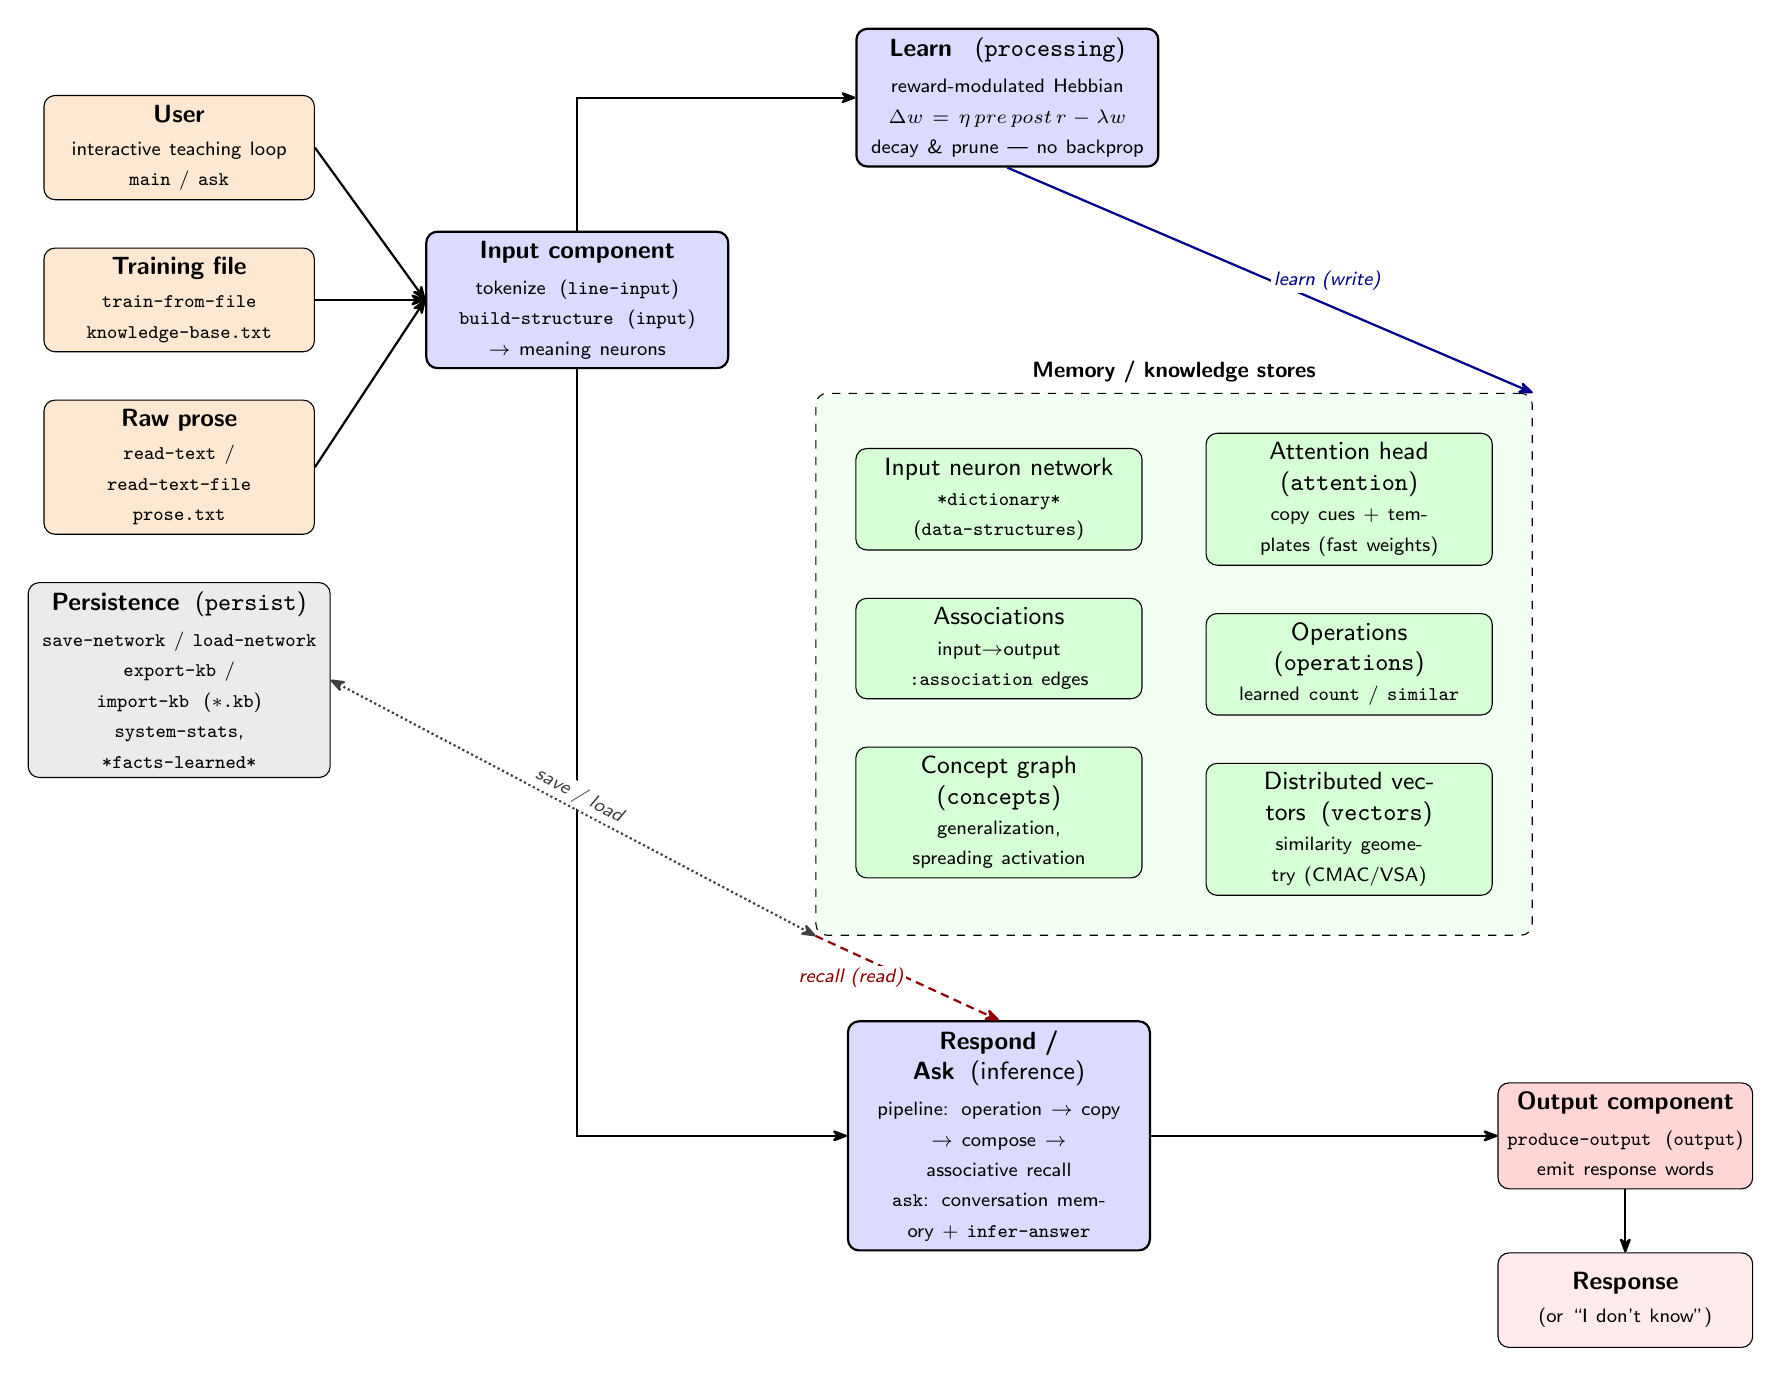
\begin{tikzpicture}[
    font=\sffamily\small,
    >={Stealth[round]},
    node distance=6mm,
    src/.style   ={draw, rounded corners, fill=orange!18, align=center,
                   text width=32mm, minimum height=12mm},
    proc/.style  ={draw, rounded corners, thick, fill=blue!14, align=center,
                   text width=36mm, minimum height=12mm},
    store/.style ={draw, rounded corners, fill=green!16, align=center,
                   text width=34mm, minimum height=9mm},
    io/.style    ={draw, rounded corners, fill=red!16, align=center,
                   text width=30mm, minimum height=12mm},
    side/.style  ={draw, rounded corners, fill=gray!16, align=center,
                   text width=36mm, minimum height=12mm},
    lbl/.style   ={font=\sffamily\scriptsize\itshape, fill=white, inner sep=1pt},
    flow/.style  ={->, thick},
    write/.style ={->, thick, blue!55!black},
    read/.style  ={->, thick, red!55!black, densely dashed},
  ]

  % ---------------------------------------------------------------- sources ---
  \node[src] (user)  {\textbf{User}\\[1pt]
        {\scriptsize interactive teaching loop}\\
        {\scriptsize \texttt{main} / \texttt{ask}}};
  \node[src, below=of user]  (file)
        {\textbf{Training file}\\[1pt]
        {\scriptsize \texttt{train-from-file}}\\
        {\scriptsize \texttt{knowledge-base.txt}}};
  \node[src, below=of file]  (prose)
        {\textbf{Raw prose}\\[1pt]
        {\scriptsize \texttt{read-text} / \texttt{read-text-file}}\\
        {\scriptsize \texttt{prose.txt}}};

  % ------------------------------------------------------- input component ---
  \node[proc, right=14mm of file] (input)
        {\textbf{Input component}\\[2pt]
        {\scriptsize tokenize \;(\texttt{line-input})}\\
        {\scriptsize \texttt{build-structure} \;(\texttt{input})}\\
        {\scriptsize $\rightarrow$ meaning neurons}};

  % --------------------------------------------------------------- learn ---
  \node[proc, above right=8mm and 16mm of input] (learn)
        {\textbf{Learn} \;\;(\texttt{processing})\\[2pt]
        {\scriptsize reward-modulated Hebbian}\\
        {\scriptsize $\Delta w=\eta\,pre\,post\,r-\lambda w$}\\
        {\scriptsize decay \& prune --- no backprop}};

  % ------------------------------------------------------- memory stores ---
  \node[store, below right=10mm and 16mm of input] (innet)
        {Input neuron network\\{\scriptsize \texttt{*dictionary*} \;(\texttt{data-structures})}};
  \node[store, below=of innet] (assoc)
        {Associations\\{\scriptsize input$\rightarrow$output \texttt{:association} edges}};
  \node[store, below=of assoc] (concept)
        {Concept graph \;(\texttt{concepts})\\{\scriptsize generalization, spreading activation}};
  \node[store, right=8mm of innet] (attn)
        {Attention head \;(\texttt{attention})\\{\scriptsize copy cues + templates (fast weights)}};
  \node[store, below=of attn] (ops)
        {Operations \;(\texttt{operations})\\{\scriptsize learned \texttt{count} / \texttt{similar}}};
  \node[store, below=of ops] (vec)
        {Distributed vectors \;(\texttt{vectors})\\{\scriptsize similarity geometry (CMAC/VSA)}};

  \begin{scope}[on background layer]
    \node[draw, dashed, rounded corners, fill=green!5, inner sep=5mm,
          fit=(innet)(assoc)(concept)(attn)(ops)(vec)] (mem) {};
  \end{scope}
  \node[font=\sffamily\bfseries\footnotesize, anchor=south]
        at (mem.north) {Memory / knowledge stores};

  % ------------------------------------------------- respond / inference ---
  \node[proc, below=18mm of concept] (respond)
        {\textbf{Respond / Ask} \;(inference)\\[2pt]
        {\scriptsize pipeline: operation $\rightarrow$ copy}\\
        {\scriptsize $\rightarrow$ compose $\rightarrow$ associative recall}\\
        {\scriptsize \texttt{ask}: conversation memory + \texttt{infer-answer}}};

  % -------------------------------------------------------- output / reply ---
  \node[io, right=44mm of respond] (output)
        {\textbf{Output component}\\[2pt]
        {\scriptsize \texttt{produce-output} \;(\texttt{output})}\\
        {\scriptsize emit response words}};
  \node[io, fill=red!8, below=8mm of output] (reply)
        {\textbf{Response} \\[1pt]{\scriptsize (or ``I don't know'')}};

  % ----------------------------------------------------------- persistence ---
  \node[side, below=of prose] (persist)
        {\textbf{Persistence} \;(\texttt{persist})\\[2pt]
        {\scriptsize \texttt{save-network} / \texttt{load-network}}\\
        {\scriptsize \texttt{export-kb} / \texttt{import-kb} \;($\ast$\texttt{.kb})}\\
        {\scriptsize \texttt{system-stats}, \texttt{*facts-learned*}}};

  % ===================================================== edges ================
  % sources -> input
  \draw[flow] (user.east)  -- (input.west);
  \draw[flow] (file.east)  -- (input.west);
  \draw[flow] (prose.east) -- (input.west);

  % input -> learn ; input -> respond  (the same parsed input feeds both)
  \draw[flow] (input.north) |- (learn.west);
  \draw[flow] (input.south) |- (respond.west);

  % learn WRITES into the memory stores
  \draw[write] (learn.south) -- (mem.north east)
        node[lbl, midway, right]{learn (write)};

  % respond READS from the memory stores
  \draw[read]  (mem.south west) -- (respond.north)
        node[lbl, midway, left]{recall (read)};

  % respond -> output -> reply
  \draw[flow] (respond.east) -- (output.west);
  \draw[flow] (output.south) -- (reply.north);

  % persistence saves/loads the whole memory graph
  \draw[<->, thick, gray!50!black, densely dotted] (persist.east) -- (mem.south west)
        node[lbl, midway, above, sloped]{save / load};

\end{tikzpicture}
\end{document}
